\section{Grundlagen}
In diesem Kapitel werden Grundlagen erläutert, die aufgrund des interdisziplinären Charakters dieser dieser Bachelorarbeit benötigt werden um sowohl informatikbezogene und nicht informatikbezogene Aspekte zu verstehen. Diese Grundlagen sorgen für ein tieferes Verständnis des Autismus Spektrums, des Mimikry Phänomens, der während der Studie benutzten Forschungsmethoden und den technischen Grundlagen. Die Auswahl der Forschungsmethoden wird in dem Kapitel 5, Evaluierung begründet. Die restlichen Grundlagen können als eine Erweiterung des Kapitels 1, Motivation gesehen werden. 

\subsection{Autismus-Spektrum-Störung}
Autismus-Spektrum-Störung beeinträchtigt die kognitiven Empathiekomponente, d.h. Menschen mit einer Autismus-Diagnose haben Schwierigkeiten, die Perspektive einer anderen Person einzunehmen und Emotionen anderer anhand von Gestik oder Mimik zu erkennen. Dadurch entstehen Defizite im sozio-emotionalen Bereich. Diese Defizite können sich in einem reduzierten oder unerwarteten Verhalten manifestieren. Verschiedene Formen des IT-gestützten Training werden seit mehr als 10 Jahren dazu verwendet, die Defizite in dem Feld der Emotionserkennung auszugleichen~\cite{ZirkusDelfi}.

\subsection{Mimikry als Phänomen}
Das Mimikry Phänomen bezeichnet ein Verhaltensmuster, in dem Menschen in sozialer Interaktion andere Menschen unbewusst und automatisch nachahmen. Die Mimik und Körpersprache werden imitiert, was die Beziehung zwischen beteiligten Personen beeinflusst~\cite{Di01}. Das Nachahmen von Jemandem kann dazu führen, dass die Person, die nachgeahmt wird, eine bessere Beziehung zu der nachahmenden Person aufbaut~\cite{Ch02} oder eher zur Kooperation überzeugt werden kann~\cite{Sw03}. Da Menschen mit ASS Emotionserkennungs- und Nachahmungsdefizite aufweisen, könnte es den Alltag negativ beeinflussen. Das Mimikry Modul, das in dieser Bachelorarbeit implementiert und evaluiert wird, versucht die Defizite durch ein gezieltes computergestütztes Training von Mimikry auszugleichen.

\subsection{Forschungsmethoden}
Die Fragebögen zu User Experience und Usability werden im Kapitel 5, Evaluierung beschrieben.
\subsubsection{User Experience}
User Experience bewertet Variablen zur Evaluation wie Verständlichkeit der Software, Funktionalität (Reliabilität), Grad der Bedienbarkeit.
Darunter sind auch ästhetische und emotionale Faktoren zu verstehen. Eine ansprechende, „begehrenswerte” Gestaltung, Aspekte der Vertrauensbildung oder Spaß bei der Nutzung (Joy of use) zählen auch dazu, dieser Ansatz umfasst das gesamte Nutzungserlebnis~\cite{UX}. Es werden Variablen wie Attraktivität, Durchschaubarkeit, Stimulation, Originalität und Effizienz der Software untersucht.

\subsubsection{Usability}
Per Definition ist Usability das Ausmaß, in dem ein Produkt durch bestimmte Benutzer in einem bestimmten Nutzungskontext genutzt werden kann, um bestimmte Ziele effektiv, effizient und zufriedenstellend zu erreichen~\cite{ISO9241}. Es wird vor allem Gebrauchstauglichkeit, also Usablility, untersucht. Usability kann als Teil von UX gesehen werden.
\begin{flushright}
\rightskip=1.8cm\textit{``Usability ist der Grad an Qualität, in welchem der Benutzer die Interaktion mit etwas erlebt.''} \\
\vspace{.2em}
\rightskip=.8cm---Jakob Nielsen
\end{flushright}
\vspace{1em}
\noindent

\subsection{Game Based Learning}
Aus der wachsenden Popularität von Computerspielen ist die Game-Based Learning Forschungsrichtung entstanden. Game Based Learning bezeichnet alternative, computergestützte Lernquellen. Sie werden besonders von Gruppen geschätzt, die ungewöhnlich Informationen bearbeiten und denken. Die GBL-Quellen bieten zahlreiche Möglichkeiten an und ist bei den meisten Nutzern sehr beliebt~\cite{Prensky2003DigitalGL}.
Aus diesen Gründen wurde GBL erforscht. Die Anwendung der GBL Prinzipien hat sich auf die Fokussierung der Aufmerksamkeit als nützlich herausgestellt, was wieder einen positiven Einfluss auf Wirksamkeit des Lernprozesses hatte. 
\paragraph{Digitale Einheimische.}Kinder und Jugendliche können gegenwärtig als digital natives (digitale Einheimische) bezeichnet werden. Darunter versteht man, dass sie sich in einer digitalen Welt sehr wohl („wie zu Hause“) fühlen~\cite{Turula.2010}. 
Spielbasierte Lernquellen ermöglicht erreichen von neuem Publikum. Es handelt sich um Lerngruppen, die von den herkömmlichen Lernmethoden weniger profitieren~\cite{Prensky2003DigitalGL}.
\paragraph{GBL Prinzipien.}
In Fokus von GBL steht der Nutzer und seine Interaktionen mit der Software. Das Spielerlebnis sollte möglichst gut sein, um die Aufmerksamkeit auf das Spiel zu lenken und um zur Fortsetzung des Spiels zu ermutigen. Eine große Rolle bei GBL spielt dabei die Attraktivität des Spiels. Auch wenn das therapeutisches Ziel an sich als sinnvoll erscheint, kann der Lerneffekt durch eine nicht optimale Umsetzung verhindert werden. 
Durch Anwendung der GBL Prinzipien ist ein Versuch den Erwartungen und Bedürfnisse von Menschen entgegen zukommen. Die Software sollte vor allem ein positives Benutzererlebnis hinterlassen. Während einer Untersuchung der Eignung werden folgende Aspekte zu beachten, die das Benutzererlebnis beeinflussen:
\begin{enumerate}
    \item Das Programm sollte stabil laufen, es darf nicht unerwartet wegen eines Fehlers (sog. bugs) schließen~\cite{Shiratuddin2011DesigningUE}.
    \item Das Programm sollte benutzerfreundlich entwickelt werden - dabei werden UX und Usability besonders relevant~\cite{Shiratuddin2011DesigningUE}.
\end{enumerate}

\subsection{Technische Grundlagen}
\paragraph{{Zusammenarbeit mit dem Fraunhofer Institut - SHORE$^\text{\textregistered}$}}
Die Feinkonzeption des Mimikry-Moduls benötigte eine Face Recognition Software. 
Die Universität Potsdam und das Fraunhofer Institut haben schon in der Vergangenheit an einigen Projekten zusammengearbeitet. Dank der erfolgreichen Kooperation hatte UP die Möglichkeit, im Rahmen der wissenschaftlichen Forschung SHORE\re - Bildanalyse Software anzuwenden. 
Die Softwarebibliothek ''SHORE\re ermöglicht eine effiziente Analyse von Personen in Videos, hinsichtlich Geschlecht, Alter und gezeigten Emotionen''~\cite{shore}. Die Software wird für Marktanwendungen, Fahrerassistenz-Systeme und in der Medizin verwendet~\cite{shore}.

Die intelligente Echtzeitanalyse ist in der Lage, zahlreiche Merkmale dynamisch zu erkennen. Die Version, mit der die Implementierung erfolgte, besaß eine Fähigkeit folgende vier Emotionen zu erkennen
\begin{enumerate}
    \item Glücklich
    \item Traurig
    \item Überrascht
    \item Ärgerlich
\end{enumerate}

Außerdem kann die Software auch das Geschlecht (Männlich/Weiblich) und das Alter abschätzen~\cite{Kueblbeck} .

Auf den Abbildungen \ref{shore_happy} und \ref{shore_angry} sind Bilder aus der öffentliche Version der SHORE\re Software zu sehen, auf den die Ergebnisse der Echtzeitanalyse angezeigt werden. 
In dem Sichtfeld der Kamera werden die charakteristischen Merkmale gesammelt und zusammen mit ihrer Position und Lage innerhalb von zirka 1/16 einer Sekunde (basierend auf den während der Studie gesammelten Daten und Beobachtungen, kann es aber Hardware abhängig sein und sollte beim Bedarf bestätigt werden) analysiert.

\begin{figure}[!ht]
\centering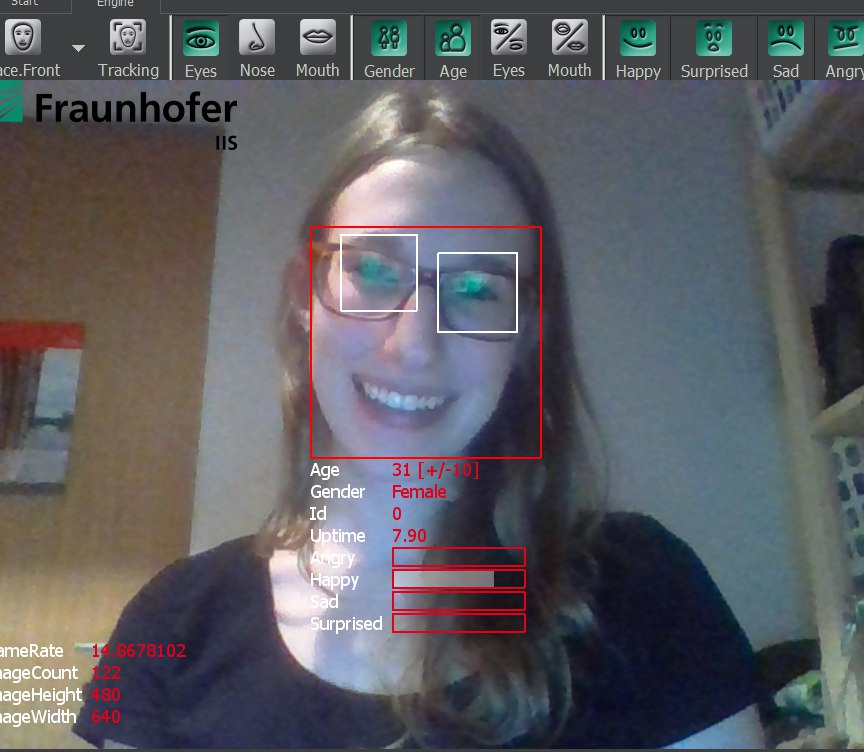
\includegraphics[width=330pt]{texes/shore_happy.png}
\caption{Hier wurden das Geschlecht der Versuchsperson (weiblich) und das Alter(26) korrekt geschätzt (mit der Abweichung +/- 10 Jahren)}
\label{shore_happy}
\end{figure}

\begin{figure}[!ht]
\centering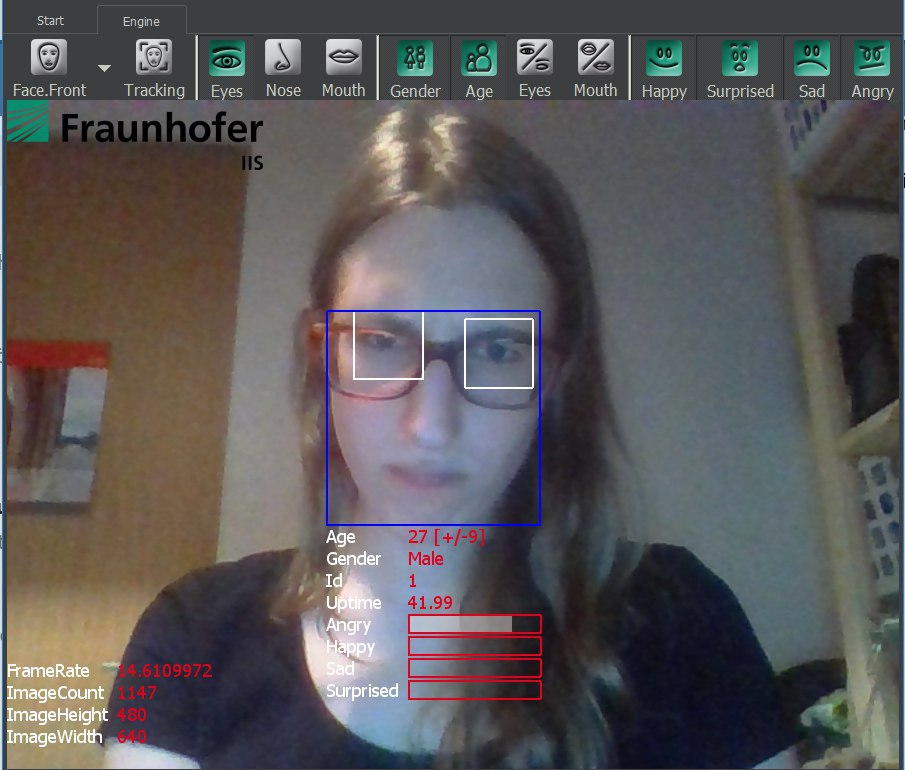
\includegraphics[width=330pt]{texes/shore_angry.png}
\caption{Ein anderer Gesichtsausdruck mit dem gleichen Rahmenbedingungen wie bei der Abb.\ref{shore_happy}. Hier wurden das Geschlecht (weiblich) falsch, dafür der Alter (26 bei der Versuchsperson) nicht nur richtig sondern auch präziser geschätzt (mit einer Abweichung von +/-9 Jahren).}
\label{shore_angry}
\end{figure}

Die Software ist plattformunabhängig und hat sehr geringe \\Hardwareanforderungen, was bei dem Entwurf des Konzepts für die eigentliche Anwendung wichtig war - geringe Harwareanforderungen bedeuten einen Zugang zu dem computergestützten Training für eine größere Menge an Patienten im Unterschied zur Software, die nur auf den neuesten Geräten funktionsfähig ist. SHORE\re funktioniert offline, die Patienten können also in einem Wartezimmer oder an einem anderen ruhigeren Ort sich befinden ohne bestehender Internetverbindung~\cite{shore}. 
Die Analyse findet auf dem Gerät statt und damit bleibt unter Kontrolle des Anwenders~\cite{shore_datenschutz}.
Die Beleuchtung und Kamerawinkel beeinflussen die Emotionsanalyse. Die optimale Ergebnisse werden bei gleichmäßig ausgeleuchteten frontalen Gesichtern erreicht.

Die Software SHORE wurde nach dem Prinzip ''Privacy by Design'' implementiert.
Aus dem System kommen nur anonyme Metainformationen heraus.
Zu den anonymen Metainformationen gehören:
\begin{enumerate}
\item Anzahl von Personen
\item Alter
\item Geschlecht
\item Gesichtsausdruck
\item Stimmung der Personen
\item Verweildauer von Personen
\end{enumerate}
Es ist aber nicht möglich festzustellen, ob eine spezifische Person schon erkannt wurde oder nicht. 
Es werden keine personenspezifische Daten aufgezeichnet, die Daten werden zwar kurzfristig gesammelt und analysiert, aber dann sofort verworfen und anonymisiert. Damit ist es unmöglich, Rückschlüsse auf die individuelle Personen zu ziehen
~\cite{Kueblbeck}.

\subsection{Konzepte aus der Android-Entwicklung}
Android-Entwicklung ist ein spezialisierter Bereich der mobilen Software Entwicklung. In diesem Abschnitt werden einige fachspezifischen Konzepte und Begrifflichkeiten, vor allem Strukturen zum Speichern von Daten erklärt, die einige für das Verständnis nützlichen Grundlagen einleiten.
Weitere Grundkonzepte der Programmierung befinden sich im Appendix.

\paragraph{Android Studio.} Die Umsetzung erfolgte mittels der Android Studio. Diese Entwicklungsumgebung ist ein in der Industrie etablierter Standard für Entwicklung von Android Apps und beinhaltet viele für Programmierer nützliche Funktionen. Mehrere Programmiersprachen werden von Android Studio benutzt, die Entwicklung des Mimikry Moduls erfolgte in Java und XML. Mit Java werden Funktionalitäten implementiert und in XML die zugehörigen Layouts erstellt.

\paragraph{SharedPreferences.}Eine Datenstruktur, die das Laden und Speichern von Schlüssel/Wert Paaren ermöglicht. Die Daten werden auf dem Gerät permanent gespeichert und sind auch nach dem Neustart verfügbar. SharedPreferences werden aufgrund der Einfachheit des Speicherns und der Möglichkeit des einfachen Ladens von überall in der App heraus benutzt.

\paragraph{Room.}Die Anwendung dieser lokalen Datenbank wurde vor der Studienphase umgesetzt um die Fortsetzung im Rahmen einer Abschlussarbeit zu ermöglichen.

\paragraph{Callbacks.} wurden hier implementiert um die Übergabe von Daten zwischen Aktivitäten und Fragmenten zu ermöglichen.
